\documentclass{beamer}
\usetheme{Madrid} % clean and academic

\usepackage[utf8]{inputenc}
\usepackage{graphicx}
\usepackage{hyperref}
\usepackage{caption}
\usepackage{subcaption}
\usepackage{amsmath, amssymb}

\title[Kuspace]{Interactive User Environment Application on Kubernetes Platform}
\author{Chalvatzis Kyriakos}
\institute{
\includegraphics[height=1cm]{Images/TUC_logo_circle.png} \\ TUC}
\date{\today}

\newcommand{\committee}{
  \begin{tabular}{ll}
    \textbf{Supervisor:} & Prof. Vasilis Samoladas \\
    \textbf{Committee:} & Prof. Nikos Giatrakos \\
                        & Prof. Euripides Petrakis \\
  \end{tabular}
}


\begin{document}

% Title Slide
\begin{frame}
  \titlepage
\end{frame}

\begin{frame}{Thesis Committee}
  \committee
\end{frame}

% Outline
\begin{frame}{Outline}
  \tableofcontents
\end{frame}

\section{Introduction}
\begin{frame}{Background}
  \begin{itemize}
    \item Data analytics has become essential across all fields — but entry-level users often struggle with the required infrastructure.
    \item Motivation: Lower the barrier for non-experts to explore and process data using standard tools. User-friendly analytical computing!
    \item While systems like Apache Spark, Airflow, and Hadoop are powerful, they are built for experienced engineers.
    \item No current open system provides isolated, user-scoped, web-accessible environments on Kubernetes — tailored for batch analytics.
  \end{itemize}
\end{frame}


\section{Objectives}
\begin{frame}{Goals}
  \begin{itemize}
    \item Although not a research thesis, this work aims to prototype a full-stack system that provides:
    \begin{itemize}
      \item Secure, multi-user access
      \item Data upload and sharing capabilities
      \item Batch job execution in a Kubernetes-native way
      \item Integrated application-like tools such as DuckDB, Python Pandas, Octave and more can be applied on datasets
    \end{itemize}
    \item Goal: Deliver an introductory platform for data analytics without overwhelming users.
    \item Goal: Achieve a Cloud-native and modular design.
  \end{itemize}
\end{frame}


\section{Methodology}
\begin{frame}{System Architecture}
  \begin{itemize}
    \item Microservice-based architecture deployed on Kubernetes
      \begin{itemize}
        \item Why? "Seperation of Concerts", scalable, modular and adaptable
      \end{itemize}
    \item Core components:
    \begin{itemize}
      \item \textbf{Uspace API}: User-facing logic for datasets, jobs, resources
      \item \textbf{FsLite}: Virtual filesystem abstraction with permissions
      \item \textbf{MinIO}: Object storage backend
      \item \textbf{Minioth}: Authentication and group-based access control
      \item \textbf{FrontApp}: Web frontend (HTML templates, HTMX, WebSocket integration)
    \end{itemize}
    \item Technologies: Go, Gin, Kubernetes, Docker
  \end{itemize}
\end{frame}

\begin{frame}{Goals 2} 
  What we want to achieve in this system:
  \begin{itemize}
    \item Identity - (Authentication) 
    \item Secure Access - (Authorization) 
    \item Physical Storage - (Data Storage)
    \item Job execution mechanism - (Job Flow)
  \end{itemize}
\end{frame}


\begin{frame}{System Diagram}
  \centering
  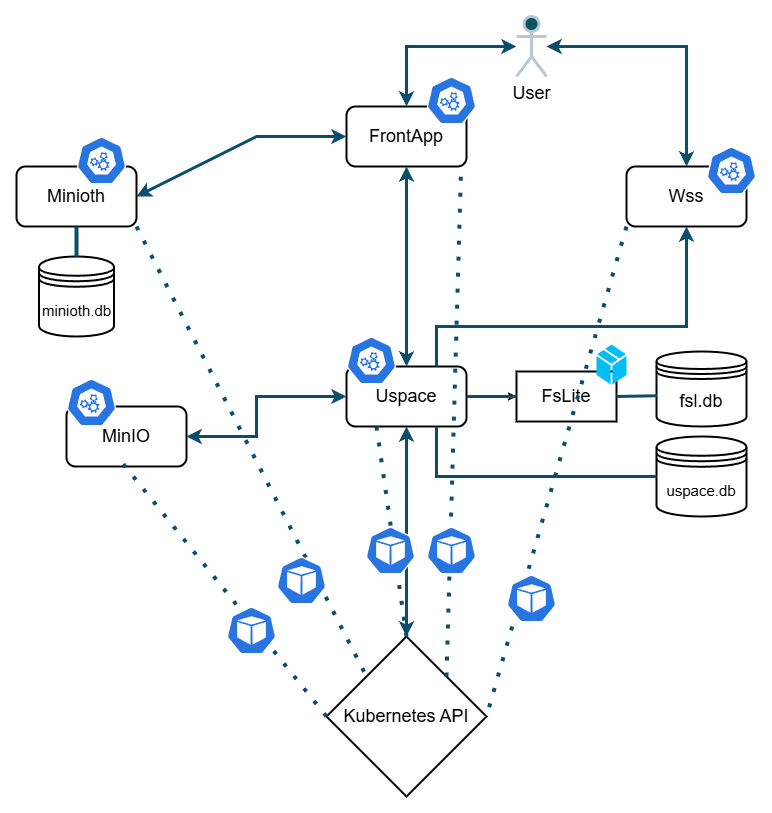
\includegraphics[width=0.5\textwidth]{Images/kuspace-overview.png}
\end{frame}

\begin{frame}{Uspace Storage Control }
  \centering
  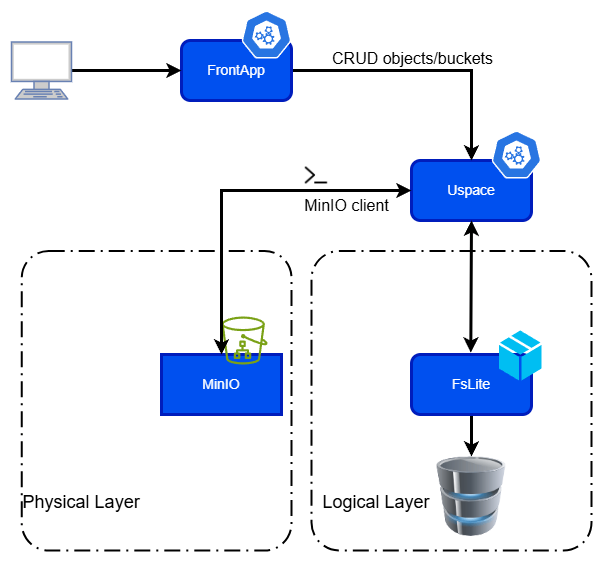
\includegraphics[width=0.6\textwidth]{Images/UspaceBlockDiagram.drawio.png}
  \captionof{figure}{UspaceStorage}
\end{frame}

\begin{frame}{Uspace Job Lifecycle}
  \centering
  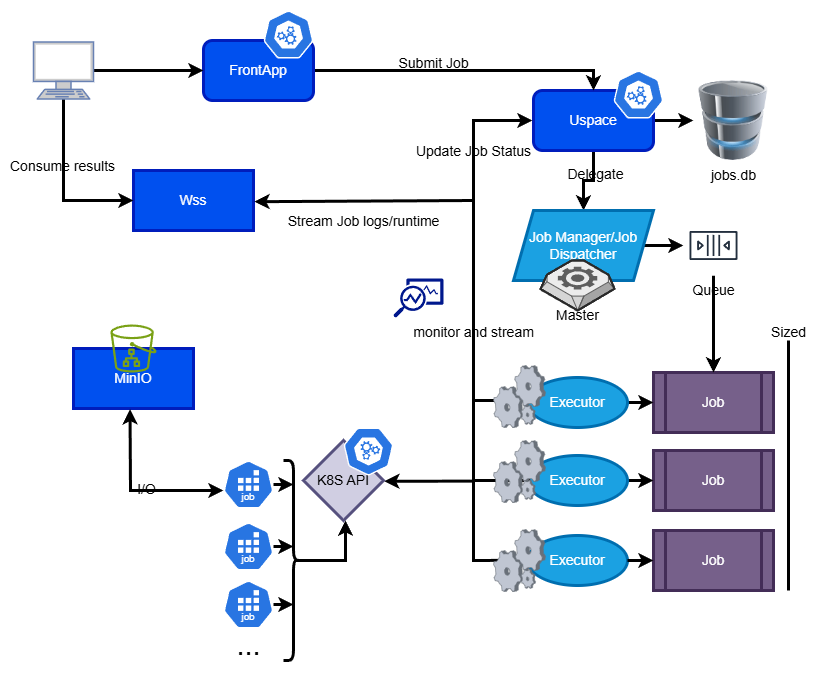
\includegraphics[width=0.7\textwidth]{Images/job-lifecycle.png}
  \captionof{figure}{Uspace Jobs}
\end{frame}

\begin{frame}{FsLite Structure}
  \centering
  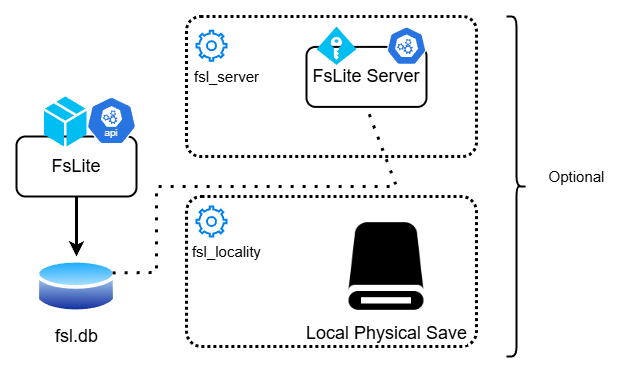
\includegraphics[width=0.7\textwidth]{Images/fsl.png}
\end{frame}

\begin{frame}{Minioth Structure}
  \centering
  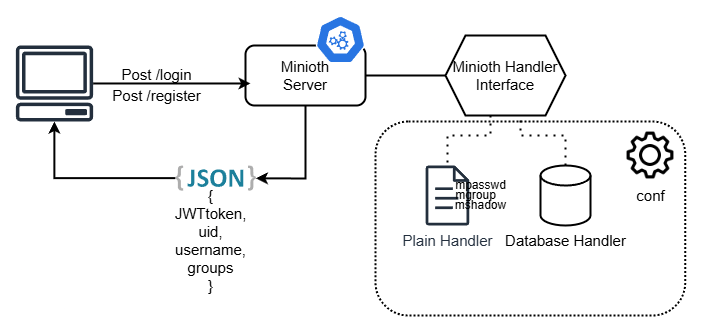
\includegraphics[width=0.7\textwidth]{Images/minioth-blockdiagram.png}
\end{frame}

\begin{frame}{Frontapp Structure}
  \centering
  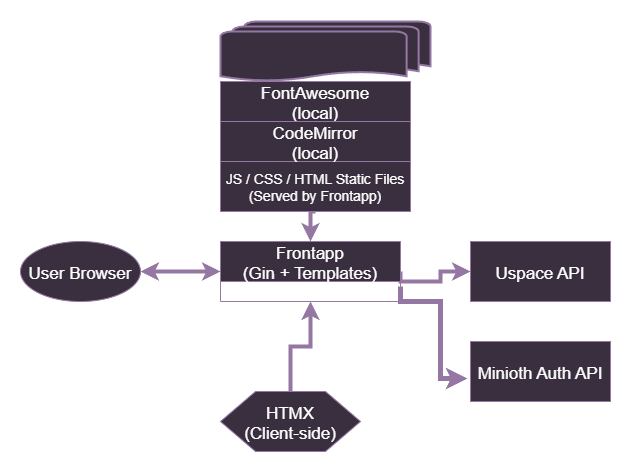
\includegraphics[width=0.7\textwidth]{Images/frontapp-blockdiagram.png}
\end{frame}

\begin{frame}{Uspace API 1}
\begin{table}[H]
\centering
\resizebox{\textwidth}{!}{%
\begin{tabular}{|l|l|p{9cm}|c|}
\hline
\textbf{Method} & \textbf{Path} & \textbf{Description} & \textbf{Requires \texttt{Access-Target}} \\
\hline
GET & \texttt{/healthz} & Health check endpoint. & No \\
GET/POST & \texttt{/api/v1/job} & Submit or list jobs. & No \\
GET/POST & \texttt{/api/v1/app} & List available tools (applications). & No \\
GET & \texttt{/api/v1/resources} & List resources (“ls” equivalent). & Yes \\
POST & \texttt{/api/v1/resource/upload} & Upload a new resource file. & Yes \\
GET & \texttt{/api/v1/resource/preview} & Preview a resource. & Yes (Read) \\
GET & \texttt{/api/v1/resource/download} & Download a resource. & Yes (Read) \\
DELETE & \texttt{/api/v1/resource/rm} & Delete a resource. & Yes (Write) \\
POST & \texttt{/api/v1/resource/cp} & Copy a resource. & Yes (Read) \\
PATCH & \texttt{/api/v1/resource/mv} & Move/rename a resource. & Yes (Write) \\
PATCH & \texttt{/api/v1/resource/permissions} & Change resource permissions. & Yes (Owner) \\
PATCH & \texttt{/api/v1/resource/ownership} & Change resource ownership. & Yes (Owner) \\
PATCH & \texttt{/api/v1/resource/group} & Change associated group. & Yes (Owner) \\
\hline
\end{tabular}
}
\caption{Uspace User API Endpoints}
\label{tab:uspace-user-endpoints}
\end{table}

\end{frame}
\begin{frame}{Uspace API 2}
  \begin{table}[H]
  \centering
  \resizebox{\textwidth}{!}{%
  \begin{tabular}{|l|l|p{9cm}|}
    \hline
    \textbf{Method} & \textbf{Path} & \textbf{Description} \\
    \hline
    GET/POST/PUT/DELETE/PATCH & \texttt{/api/v1/admin/volumes} & Full volume management API. \\
    DELETE/PUT & \texttt{/api/v1/admin/job} & Administrative job control (e.g., delete jobs). \\
    GET/POST/PATCH/DELETE & \texttt{/api/v1/admin/user/volume} & Manage user-volume mappings. \\
    GET/POST/PUT/DELETE & \texttt{/api/v1/admin/app} & Manage available applications/tools. \\
    GET & \texttt{/api/v1/admin/system-conf} & View current system configuration. \\
    GET & \texttt{/api/v1/admin/system-metrics} & System metrics via Kubernetes API. \\
    \hline
    \end{tabular}
  }
  \caption{Uspace Admin API Endpoints}
  \end{table}

\end{frame}

\begin{frame}{FsLite API}
  
\begin{table}[H]
  \centering
  \resizebox{\textwidth}{!}{%
  \begin{tabular}{|l|l|p{9cm}|}
  \hline
  \textbf{Method} & \textbf{Path} & \textbf{Description}\\
  \hline
  \hline
  POST              & \texttt{/login}                     & Authenticate and receive a token.\\
  POST              & \texttt{/admin/register}            & Authenticate and receive JWT token.\\
  POST              & \texttt{/admin/volume/new}          & Change password for the authenticated user.\\
  DELETE            & \texttt{/admin/volume/delete}       & Delete a specified volume\\
  GET               & \texttt{/admin/volume/get}          & Retrieve information about a logical volume\\
  GET               & \texttt{/admin/resource/get}        & Retrieve metadata of multiple resources \\ 
  GET               & \texttt{/admin/resource/stat}       & Retrieve more detailed metadata of a specific resource.\\
  DELETE            & \texttt{/admin/resource/delete}     & Delete a specified resource.\\
  POST              & \texttt{/admin/resource/upload}     & Upload resource content to volume.\\
  GET               & \texttt{/admin/resource/download}   & Download a resource from storage.\\
  GET/PATCH/DELETE  & \texttt{/admin/user/voumes}         & CRUD user volumes.\\
  \hline
  \hline
  \end{tabular}%
  }
  \caption{FsLite public API endpoints}
  \label{tab:fslite-public-endpoints}
\end{table}
\end{frame}

\begin{frame}{Minioth API 1}
  \begin{table}[H]
\centering
\resizebox{\textwidth}{!}{%
\begin{tabular}{|l|l|p{7cm}|c|}
\hline
\textbf{Method} & \textbf{Path} & \textbf{Description} & \textbf{Auth} \\
\hline
\hline
POST  & \texttt{/v1/register}            & Register a new user.                           & No  \\
POST  & \texttt{/v1/login}               & Authenticate and receive JWT token.            & No  \\
POST  & \texttt{/v1/passwd}              & Change password for the authenticated user.    & Yes (user/admin) \\
GET   & \texttt{/v1/user/me}             & Get information about the token's user.        & Token \\
GET   & \texttt{/v1/user/token}          & View current token details.                    & No \\
POST  & \texttt{/v1/user/refresh-token}  & Request a new access token using a refresh token. & No \\
GET   & \texttt{/v1/swagger/*any}        & Swagger UI for live API documentation.         & No \\
\hline
\hline
\end{tabular}%
}
\caption{Minioth public/user API endpoints}
\label{tab:minioth-public-endpoints}
\end{table}
\end{frame}

\begin{frame}{Minioth API 2}
\begin{table}[H]
\centering
\resizebox{\textwidth}{!}{%
\begin{tabular}{|l|l|p{7cm}|c|}
\hline
\textbf{Method} & \textbf{Path} & \textbf{Description} \\
\hline
\hline
GET    & \texttt{/v1/admin/audit/logs}      & Retrieve system audit logs. \\
POST   & \texttt{/v1/admin/hasher}          & Generate bcrypt hashes from plaintext passwords. \\
POST   & \texttt{/v1/admin/verify-password} & Compare a password against a stored hash. \\
GET    & \texttt{/v1/admin/users}           & List all registered users. \\
GET    & \texttt{/v1/admin/groups}          & List all groups and their members. \\
POST   & \texttt{/v1/admin/useradd}         & Add a new user to the system. \\
DELETE & \texttt{/v1/admin/userdel}         & Delete a user by UID or username. \\
PATCH  & \texttt{/v1/admin/userpatch}       & Update selected fields of a user. \\
PUT    & \texttt{/v1/admin/usermod}         & Fully replace a user record. \\
POST   & \texttt{/v1/admin/groupadd}        & Create a new group. \\
PATCH  & \texttt{/v1/admin/grouppatch}      & Update specific fields of a group. \\
PUT    & \texttt{/v1/admin/groupmod}        & Fully update a group definition. \\
DELETE & \texttt{/v1/admin/groupdel}        & Remove a group from the system. \\
POST   & \texttt{/v1/admin/rotate}          & Rotate the JWT signing key in use. \\
GET    & \texttt{/v1/admin/system-conf}     & View current server configuration. \\
\hline
\hline
\end{tabular}%
}
\caption{Minioth public/admin API endpoints}
\end{table}

\end{frame}






\section{Results}

\begin{frame}{Demonstration \& Key Features}
  \begin{itemize}
    \item Fully functioning web interface for:
    \begin{itemize}
      \item Uploading datasets
      \item Launching batch jobs with SQL, Python, or predefined tools
      \item Viewing logs in real time (WebSocket streaming)
    \end{itemize}
    \item Example: Executing DuckDB query on uploaded CSV → result saved and downloadable
    \item Job isolation: Every job runs in its own Kubernetes Pod
  \end{itemize}
\end{frame}



\section{Conclusion}
\begin{frame}{Summary and Future Work}
  \begin{itemize}
    \item \textbf{Accomplishments}:
    \begin{itemize}
      \item Designed and implemented a user-centric data platform on Kubernetes
      \item Combined identity, authorization, storage, and batch compute layers
      \item Delivered a fully working demo with real-world tools and users
    \end{itemize}
    \item \textbf{Limitations}:
      \begin{itemize}
        \item Not expected to perform fast on really big data
      \end{itemize} 
    \item \textbf{Future Work}:
    \begin{itemize}
      \item Extend toolset: Jupyter, R, Julia, Tool For Tools
      \item Add CI/CD for job templates and data pipelines
      \item CLI tool, a road to the Shell 
      \item Distributed orchestration...
    \end{itemize}
  \end{itemize}
\end{frame}


% Final slide
\begin{frame}{Questions?}
  \centering
  \Huge Thank you! \\
  \vspace{1em}
  \normalsize
  \texttt{kchalvatzis@tuc.gr}
\end{frame}

\end{document}
